\chapter{Latches and Flip-Flops}
\label{ch:latch}

Combinational circuits forget: the moment their inputs change, their old outputs are gone. But a computer must remember things: the value in a register, the count in a counter, which step a machine is on. This chapter builds memory out of gates. It explains latches and flip-flops, the difference between them (an assessment question), how to build a flip-flop from multiplexers (an interview question), and the strange behavior called metastability.

\section{Memory from feedback}

Connect two inverters in a loop: the output of the first drives the second, and the output of the second drives the first (Figure~\ref{fig:bistable}).

\begin{figure}[h]
\centering
\begin{circuitikz}
  \draw (0,0) node[not port](a){};
  \draw (0,-1.6) node[not port, xscale=-1](b){};
  \draw (a.out) -- ++(0.5,0) coordinate(q) |- (b.in);
  \draw (b.out) -- ++(-0.5,0) |- (a.in);
  \node[right] at (q) {$Q$};
  \node[left] at ($(b.out)+(-0.5,0.8)$) {$\nt{Q}$};
\end{circuitikz}
\caption{Two cross-coupled inverters: a circuit with two stable states.}
\label{fig:bistable}
\end{figure}

If $Q = 1$, the lower inverter makes $\nt{Q} = 0$, and the upper inverter turns that back into $Q = 1$. The loop holds itself. If $Q = 0$, the same reasoning shows the loop holds that too. The circuit is \term{bistable}: it has two stable states and stays in whichever one it is put in, as long as power is on. That is one bit of memory.

\begin{everyday}
A light switch is bistable: push it up and it stays up, push it down and it stays down. A doorbell button is not: it only stays pressed while you hold it. Memory circuits are the light-switch kind.
\end{everyday}

The remaining problem is how to \emph{write} a new value into the loop. Every latch and flip-flop is a bistable loop plus some way to control when it accepts new data.

\section{The SR latch}

Replace the two inverters with two NOR gates, giving each a spare input: $S$ (set) and $R$ (reset). This is the \term{SR latch} (Figure~\ref{fig:srlatch}).

\begin{figure}[h]
\centering
\begin{circuitikz}
  \draw (0,0) node[nor port](n1){};
  \draw (0,-2.4) node[nor port](n2){};
  \draw (n1.in 1) -- ++(-0.8,0) node[left]{$R$};
  \draw (n2.in 2) -- ++(-0.8,0) node[left]{$S$};
  \draw (n1.out) -- ++(0.8,0) coordinate(q) node[right]{$Q$};
  \draw (n2.out) -- ++(0.8,0) coordinate(qb) node[right]{$\nt{Q}$};
  \draw ($(n1.out)+(0.4,0)$) -- ++(0,-0.7) -- ++(-2.2,-0.6) |- (n2.in 1);
  \draw ($(n2.out)+(0.4,0)$) -- ++(0,0.7) -- ++(-2.2,0.6) |- (n1.in 2);
\end{circuitikz}
\caption{An SR latch made of two cross-coupled NOR gates.}
\label{fig:srlatch}
\end{figure}

Recall that a NOR outputs 0 whenever any input is 1.
\begin{center}
\begin{tabular}{cc|l}
\toprule
$S$ & $R$ & Result \\
\midrule
0 & 0 & hold: $Q$ keeps its previous value \\
1 & 0 & set: $Q = 1$ \\
0 & 1 & reset: $Q = 0$ \\
1 & 1 & forbidden: both outputs forced to 0 \\
\bottomrule
\end{tabular}
\end{center}

$S = R = 1$ is forbidden for two reasons: $Q$ and $\nt{Q}$ are both 0, so they are no longer opposites; and if $S$ and $R$ then drop to 0 at the same moment, the latch races to an unpredictable state. An SR latch built from NAND gates works the same way with active-low inputs ($\nt{S}$ and $\nt{R}$, where 0 means ``do it'').

\section{The D latch}

The SR latch has two awkward inputs and a forbidden case. The \term{D latch} fixes both. It has a data input $D$ and an enable $EN$ (often the clock):
\begin{itemize}
  \item While $EN = 1$, the latch is \term{transparent}: $Q$ follows $D$, changing whenever $D$ changes.
  \item While $EN = 0$, the latch is \term{opaque}: $Q$ holds whatever value $D$ had at the moment $EN$ fell.
\end{itemize}

The simplest way to build one is a 2:1 mux whose output feeds back to one of its own inputs:
\[
  Q = EN\;?\;D : Q.
\]
When $EN = 1$ the mux passes $D$; when $EN = 0$ it passes its own output back to itself, a loop that holds the value (Figure~\ref{fig:muxlatch}). In transistor-level designs, the mux is made of two transmission gates, one letting $D$ in and one closing the feedback loop of two inverters.

\begin{figure}[h]
\centering
\begin{tikzpicture}
  \muxtwo{m}{(0,0)}{}
  \draw (m-in1) -- ++(-1.0,0) node[left]{$D$};
  \draw (m-sel) -- ++(0,-0.6) node[below]{$EN$};
  \draw (m-out) -- ++(1.2,0) coordinate(q) node[right]{$Q$};
  \draw ($(m-out)+(0.6,0)$) -- ++(0,1.4) -- ++(-2.2,0) |- (m-in0);
  \fill ($(m-out)+(0.6,0)$) circle (0.05);
\end{tikzpicture}
\caption{A D latch from a 2:1 mux. The 1 input takes new data; the 0 input feeds the output back to hold it.}
\label{fig:muxlatch}
\end{figure}

\begin{figure}[h]
\centering
\begin{tikztimingtable}[timing/slope=0.05, xscale=1.6, yscale=1.2]
$EN$ & LL HHHH LLLL HHHH LL \\
$D$  & L HHH LL HH LL LLL HHH \\
$Q$  & LL HH LL LLLL LLL HHH \\
\extracode
\begin{pgfonlayer}{background}
\vertlines[help lines]{2,6,10,14}
\end{pgfonlayer}
\end{tikztimingtable}
\caption{A D latch: while $EN$ is high, $Q$ follows $D$; while $EN$ is low, $Q$ holds (the pulse on $D$ during the low phase never reaches $Q$).}
\label{fig:latchtiming}
\end{figure}

\section{The edge-triggered D flip-flop}

A latch is transparent for the whole time its enable is high, which makes timing hard to control (we will see why shortly). Usually we want a storage element that captures its input at one precise instant, the moment the clock rises, and ignores the input at all other times. That is the \term{D flip-flop}.

\paragraph{Master--slave construction.} Put two D latches in a row with opposite enables (Figure~\ref{fig:masterslave}):
\begin{itemize}
  \item the \term{master} latch is transparent while $CLK = 0$;
  \item the \term{slave} latch is transparent while $CLK = 1$.
\end{itemize}

\begin{figure}[h]
\centering
\begin{tikzpicture}
  \dbox{m}{(0,0)}{master}{0}
  \dbox{s}{(3.2,0)}{slave}{0}
  \draw (m-d) -- ++(-0.8,0) node[left]{$D$};
  \draw (m-q) -- node[above,font=\small]{$Q_m$} (s-d);
  \draw (s-q) -- ++(0.8,0) node[right]{$Q$};
  \draw (m-clk) -- ++(-0.8,0) node[left]{$\nt{CLK}$};
  \draw (s-clk) -- ++(-0.5,0) node[left]{$CLK$};
\end{tikzpicture}
\caption{A positive-edge-triggered D flip-flop: master latch enabled by $\nt{CLK}$, slave latch enabled by $CLK$.}
\label{fig:masterslave}
\end{figure}

Step through one clock cycle:
\begin{enumerate}
  \item \textbf{While $CLK = 0$:} the master is transparent, so $Q_m$ follows $D$. The slave is opaque, so $Q$ holds its old value.
  \item \textbf{At the rising edge:} the master closes, freezing $Q_m$ at the value $D$ had at that instant. At the same moment the slave opens and passes that frozen value to $Q$.
  \item \textbf{While $CLK = 1$:} the master is closed, so changes on $D$ cannot get in. The slave is transparent, but its input $Q_m$ is frozen, so $Q$ stays put.
\end{enumerate}
The net effect: $Q$ takes the value of $D$ at each rising clock edge and holds it for the rest of the cycle. At no time is there a transparent path all the way from $D$ to $Q$.

\begin{figure}[h]
\centering
\begin{tikztimingtable}[timing/slope=0.05, xscale=1.6, yscale=1.2]
$CLK$ & LL HH LL HH LL HH LL HH \\
$D$   & L HH L H LLLL HHHH LLL \\
$Q$   & LL HHHH LLLL HHHH LL \\
\extracode
\begin{pgfonlayer}{background}
\vertlines[help lines]{2,6,10,14}
\end{pgfonlayer}
\end{tikztimingtable}
\caption{A D flip-flop: $Q$ changes only at rising clock edges (gridlines), taking the value $D$ had at that instant. The brief dip in $D$ between edges is ignored.}
\label{fig:fftiming}
\end{figure}

\section{A D flip-flop from two 2:1 multiplexers}
\label{sec:ffmux}

Since a D latch is one mux with feedback, a flip-flop is two of them:

\begin{itemize}
  \item \textbf{Master mux:} $S = CLK$, $I_0 = D$, $I_1 = Q_m$ (its own output fed back). It is transparent when $CLK = 0$ and holds when $CLK = 1$.
  \item \textbf{Slave mux:} $S = CLK$, $I_0 = Q$ (its own output fed back), $I_1 = Q_m$. It holds when $CLK = 0$ and is transparent when $CLK = 1$.
\end{itemize}

\begin{figure}[h]
\centering
\begin{tikzpicture}
  \muxtwo{a}{(0,0)}{}
  \muxtwo{b}{(3.6,0)}{}
  \draw (a-in0) -- ++(-1.0,0) node[left]{$D$};
  % master feedback into in1
  \draw (a-out) -- ++(0.6,0) coordinate(am);
  \fill (am) circle (0.05);
  \draw (am) |- ($(a-in1)+(-0.5,-0.9)$) |- (a-in1);
  % master to slave in1
  \draw (am) -- ++(1.2,0) |- (b-in1);
  \node[above,font=\small] at ($(am)+(0.6,0)$) {$Q_m$};
  % slave feedback into in0
  \draw (b-out) -- ++(0.7,0) coordinate(bq);
  \fill (bq) circle (0.05);
  \draw (bq) |- ($(b-in0)+(-0.5,1.0)$) |- (b-in0);
  \draw (bq) -- ++(0.6,0) node[right]{$Q$};
  % clock
  \draw (a-sel) -- ++(0,-1.3) coordinate(ca);
  \draw (b-sel) -- ++(0,-1.3) coordinate(cb);
  \draw ($(ca)+(-1.4,0)$) node[left]{$CLK$} -- (cb);
  \fill (ca) circle (0.05);
  \node[font=\small] at (0.5,2.3) {master};
  \node[font=\small] at (4.1,2.85) {slave};
\end{tikzpicture}
\caption{A positive-edge D flip-flop from two 2:1 muxes. Both selects are driven by $CLK$; the feedback goes to opposite data inputs, so the two latches are transparent in opposite clock phases.}
\label{fig:ffmux}
\end{figure}

\begin{onoa}
Interview reports include ``make a D flip-flop using 2:1 muxes.'' The answer is Figure~\ref{fig:ffmux}: two mux-latches in series, enabled in opposite clock phases. (Moving the feedback to the other input of each mux gives a negative-edge flip-flop.) In real silicon, care is needed so that both latches are never transparent at the same time during the clock transition, but the logical structure is exactly this.
\end{onoa}

\section{Latch versus flip-flop}
\label{sec:latchvsff}

\begin{center}
\begin{tabularx}{\linewidth}{>{\raggedright\arraybackslash}p{3.2cm}>{\raggedright\arraybackslash}X>{\raggedright\arraybackslash}X}
\toprule
 & Latch & Flip-flop \\
\midrule
Triggered by & clock \textbf{level} & clock \textbf{edge} \\
While the clock is active & transparent: output follows input & opaque: input only sampled at the edge \\
Size & one latch (smaller) & two latches (about twice the size) \\
Power & lower & higher (more transistors, more clock load) \\
Glitches on the input & passed through while transparent & ignored except near the edge \\
Timing & harder: data can race through; but allows time borrowing & simpler: one capture per cycle \\
\bottomrule
\end{tabularx}
\end{center}

\begin{onoa}
``What is one advantage of a flip-flop over a latch?'' was an Ignite assessment question. The key answer: \textbf{a flip-flop is edge-triggered, so it samples its input at one instant per cycle and is never transparent.} Data cannot ``race through'' several stages in one clock phase, glitches on the input are ignored, and timing analysis is simple and predictable. Advantages of a latch in return: it is smaller, uses less power, and allows \emph{time borrowing} (a slow stage can use some of the next stage's time while the latch is transparent, Chapter~\ref{ch:timing}).
\end{onoa}

\paragraph{Why race-through is a problem.} Imagine a pipeline of latches all enabled by the same clock. While the clock is high, every latch is transparent at once, and data entering the first latch can rush through the logic and into the second, third and fourth before the clock falls. The circuit no longer advances one step per cycle; it advances an unpredictable number of steps depending on gate delays. Flip-flops cannot do this, because no flip-flop is ever transparent from input to output. (Latch-based designs avoid the problem by alternating latches on opposite clock phases, which is exactly what a master--slave flip-flop does internally.)

\section{Other kinds of flip-flop}

Older textbooks and some interview questions use other flip-flop types. Each can be built from a D flip-flop plus a little logic.

\begin{center}
\begin{tabular}{lll}
\toprule
Type & Behavior at the clock edge & Next state $Q^+$ \\
\midrule
D & copy $D$ & $D$ \\
T (toggle) & flip if $T = 1$, hold if $T = 0$ & $T \oplus Q$ \\
JK & $J$ sets, $K$ resets, both 1 toggles, both 0 holds & $J\nt{Q} + \nt{K}Q$ \\
SR & $S$ sets, $R$ resets, both 1 not allowed & $S + \nt{R}Q$ \\
\bottomrule
\end{tabular}
\end{center}

\begin{itemize}
  \item A \textbf{T flip-flop} is a D flip-flop with $D = T \oplus Q$.
  \item A \textbf{T flip-flop with $T = 1$}, or a D flip-flop with $\nt{Q}$ fed back to $D$, toggles on every clock edge. Its output is a square wave at \emph{half} the clock frequency: a divide-by-two circuit (Chapter~\ref{ch:fsm}).
\end{itemize}

\section{Set, reset and enable}

\paragraph{Asynchronous set and clear.} Many flip-flops have extra inputs that force the output immediately, without waiting for a clock edge: \term{preset} (or set) forces $Q = 1$, and \term{clear} (or reset) forces $Q = 0$. These are often \term{active low}, written $\nt{PRE}$ and $\nt{CLR}$: they act when held at 0.

\begin{trap}
``Set and clear tied to zero'' means opposite things depending on the polarity. For \emph{active-high} set and clear, tying them to 0 disables them, and the flip-flop works normally. For \emph{active-low} inputs, tying them to 0 asserts them, and the output is stuck (and with both asserted, the behavior is invalid). Always check whether the input has a bubble on the symbol.
\end{trap}

\paragraph{Synchronous versus asynchronous reset.} An \term{asynchronous} reset acts immediately, even with no clock running. A \term{synchronous} reset is just a condition in the logic in front of $D$, so it takes effect only at the next clock edge. Both are common; Chapter~\ref{ch:rtl} discusses the trade-offs.

\paragraph{Enable.} To make a flip-flop update only when an enable signal is 1, put a mux in front of it: $D_{\text{ff}} = EN\;?\;D : Q$. When disabled, the flip-flop reloads its own value each cycle. (An alternative is to stop its clock, called clock gating, which saves power, Chapter~\ref{ch:power}.)

\paragraph{Scan flip-flops.} Chips are tested after manufacturing by loading known patterns into every flip-flop. A \term{scan flip-flop} has a mux in front that, in test mode, connects all flip-flops into one long shift register (a \term{scan chain}) so test patterns can be shifted in and results shifted out.

\section{Metastability}
\label{sec:metastability}

A flip-flop needs its input to be stable for a short window around the clock edge (the setup and hold times, Chapter~\ref{ch:timing}). What if the input changes inside that window? The bistable loop can be caught balanced exactly between its two states, like a ball balanced on top of a hill. Eventually noise tips it one way or the other, but \emph{how long} that takes is unpredictable. While it hangs there, the output sits at an in-between voltage that is neither a valid 0 nor a valid 1. This is \term{metastability}.

\begin{figure}[h]
\centering
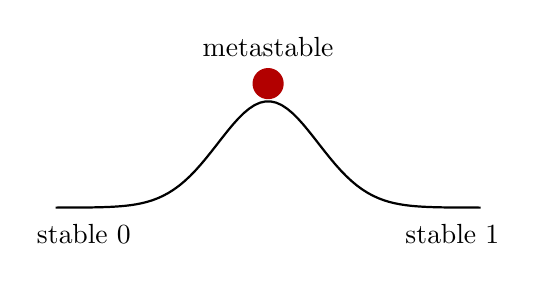
\begin{tikzpicture}[scale=0.9]
  \draw[thick,domain=-3:3,samples=80] plot (\x,{1.5*exp(-\x*\x)});
  \fill[red!70!black] (0,1.75) circle (0.22);
  \node[below] at (-2.6,-0.1) {stable 0};
  \node[below] at (2.6,-0.1) {stable 1};
  \node[above] at (0,2.0) {metastable};
\end{tikzpicture}
\caption{Metastability: a ball balanced on a hill eventually rolls to one side, but nobody can say exactly when.}
\end{figure}

Key facts:
\begin{itemize}
  \item Metastability happens whenever the input is \term{asynchronous}: it comes from outside the flip-flop's clock domain (a button, another chip, a different clock), so it can change at any time.
  \item It \emph{cannot be eliminated}, only made very unlikely.
  \item The probability that the flip-flop is still unresolved after waiting time $t$ falls \emph{exponentially} with $t$. So the mean time between failures (MTBF) grows exponentially with the time you allow it to settle.
  \item The standard defense is a \term{synchronizer}: two flip-flops in a row on the receiving clock. The first may go metastable, but it has a whole clock cycle to resolve before the second samples it. This reduces the failure rate to something like once in thousands of years (Chapter~\ref{ch:rtl}).
\end{itemize}

\section{Summary}

\begin{itemize}
  \item Memory comes from feedback: two cross-coupled inverters are bistable.
  \item SR latch: set, reset, hold; $S = R = 1$ forbidden.
  \item D latch: transparent while enabled, holds while disabled. A 2:1 mux with feedback is a D latch.
  \item D flip-flop: master latch (transparent on $CLK = 0$) plus slave latch (transparent on $CLK = 1$) captures $D$ at the rising edge. Two muxes make one.
  \item Flip-flop advantages: edge-triggered, never transparent, no race-through, glitches ignored, easy timing. Latch advantages: smaller, lower power, time borrowing.
  \item T flip-flop: $Q^+ = T \oplus Q$; with $T = 1$ it divides the clock by 2. JK: $Q^+ = J\nt{Q} + \nt{K}Q$.
  \item Check set/clear polarity before deciding what ``tied to 0'' means.
  \item Metastability cannot be eliminated; synchronizers make it exponentially unlikely.
\end{itemize}

\section{Exercises}

\begin{enumerate}
  \item A NOR SR latch has $S = 1$, $R = 0$. Then $S$ returns to 0. What is $Q$ now?
  \item Why is $S = R = 1$ not allowed in a NOR SR latch?
  \item A D latch has $EN = 1$ and $D$ toggles three times. How many times does $Q$ change? What if $EN = 0$?
  \item Draw (or describe) a D latch made from one 2:1 mux. Which input gets the feedback?
  \item Describe the connections of a positive-edge D flip-flop built from two 2:1 muxes.
  \item State one advantage of a flip-flop over a latch, and one advantage of a latch over a flip-flop.
  \item How do you make a T flip-flop from a D flip-flop?
  \item A JK flip-flop has $J = K = 1$. What does it do on each clock edge?
  \item A flip-flop has active-low asynchronous clear, and the clear input is tied to 0. What is $Q$?
  \item True or false: with careful design, metastability can be completely eliminated.
  \item A D flip-flop is clocked at 100\,MHz with $\nt{Q}$ connected to $D$. What is the frequency of $Q$?
\end{enumerate}

\subsection*{Answers}
\begin{enumerate}
  \item $Q = 1$: the latch was set, and with $S = R = 0$ it holds.
  \item It forces both $Q$ and $\nt{Q}$ to 0 (no longer complements), and if both inputs then return to 0 together, the final state depends on a race and is unpredictable.
  \item Three times (it is transparent; $Q$ follows each change of $D$). With $EN = 0$, zero times.
  \item The mux's select is $EN$; $D$ goes to the 1 input; the output is fed back to the 0 input.
  \item Master mux: select $CLK$, $I_0 = D$, $I_1$ = its own output $Q_m$. Slave mux: select $CLK$, $I_1 = Q_m$, $I_0$ = its own output $Q$.
  \item Flip-flop: edge-triggered, never transparent, so no race-through and simpler timing (also ignores glitches). Latch: smaller and lower power, and allows time borrowing.
  \item Feed $D = T \oplus Q$.
  \item It toggles ($Q^+ = \nt{Q}$).
  \item The clear is permanently asserted, so $Q$ is stuck at 0.
  \item False. Its probability can only be made extremely small.
  \item 50\,MHz (the output toggles once per clock period, so its period is two clock periods).
\end{enumerate}
